This chapter presents the methodological framework, tools, data pipeline, model design, and training protocol used to build and benchmark the proposed Alzheimer's Disease (AD) detection system. The emphasis is on \emph{how} a family of fully three-dimensional models --- a 3D CNN, a pretrained 3D ResNet, a 3D Vision Transformer (ViT), a Swin Transformer, and a hybrid 3D CNN--ViT --- was developed, trained, and evaluated on identical data and splits, so that the single-vs-hybrid comparison at the heart of this thesis is fair and reproducible.

\section{Methodological Framework}
The methodology was structured into sequential stages to ensure a systematic and leakage-free implementation. The workflow began with \textbf{problem formulation}: rather than chasing a single inflated accuracy figure, the goal was fixed as an \emph{honest, subject-level} comparison of 3D deep-learning architectures on structural MRI. Two clinically meaningful classification tasks were defined:
\begin{enumerate}
    \item \textbf{Binary CN-vs-AD} --- separating cognitively normal (CN) subjects from Alzheimer's (AD) subjects. This is the headline task, where high accuracy is genuinely achievable.
    \item \textbf{Three-class CN/MCI/AD} --- additionally distinguishing mild cognitive impairment (MCI), the transitional stage. This is reported as the harder, honest benchmark.
\end{enumerate}
\textbf{Data acquisition} used a single, authoritative source, the Alzheimer's Disease Neuroimaging Initiative (ADNI), to avoid the domain-shift and label-mismatch problems that arise when 2D and 3D datasets are mixed. \textbf{Preprocessing and data preparation} standardized every volume into a common orientation, resolution, and intensity range using MONAI transforms. In the \textbf{modelling} stage, five architectures sharing a common feature-extraction interface and classifier head were built. \textbf{Training and evaluation} were performed with five-fold subject-level cross-validation, reporting mean $\pm$ standard deviation across folds. Finally, \textbf{explainability} was applied with a suite of 3D attribution methods to verify that the models attend to anatomically plausible regions.

\begin{figure}[H]
    \centering
    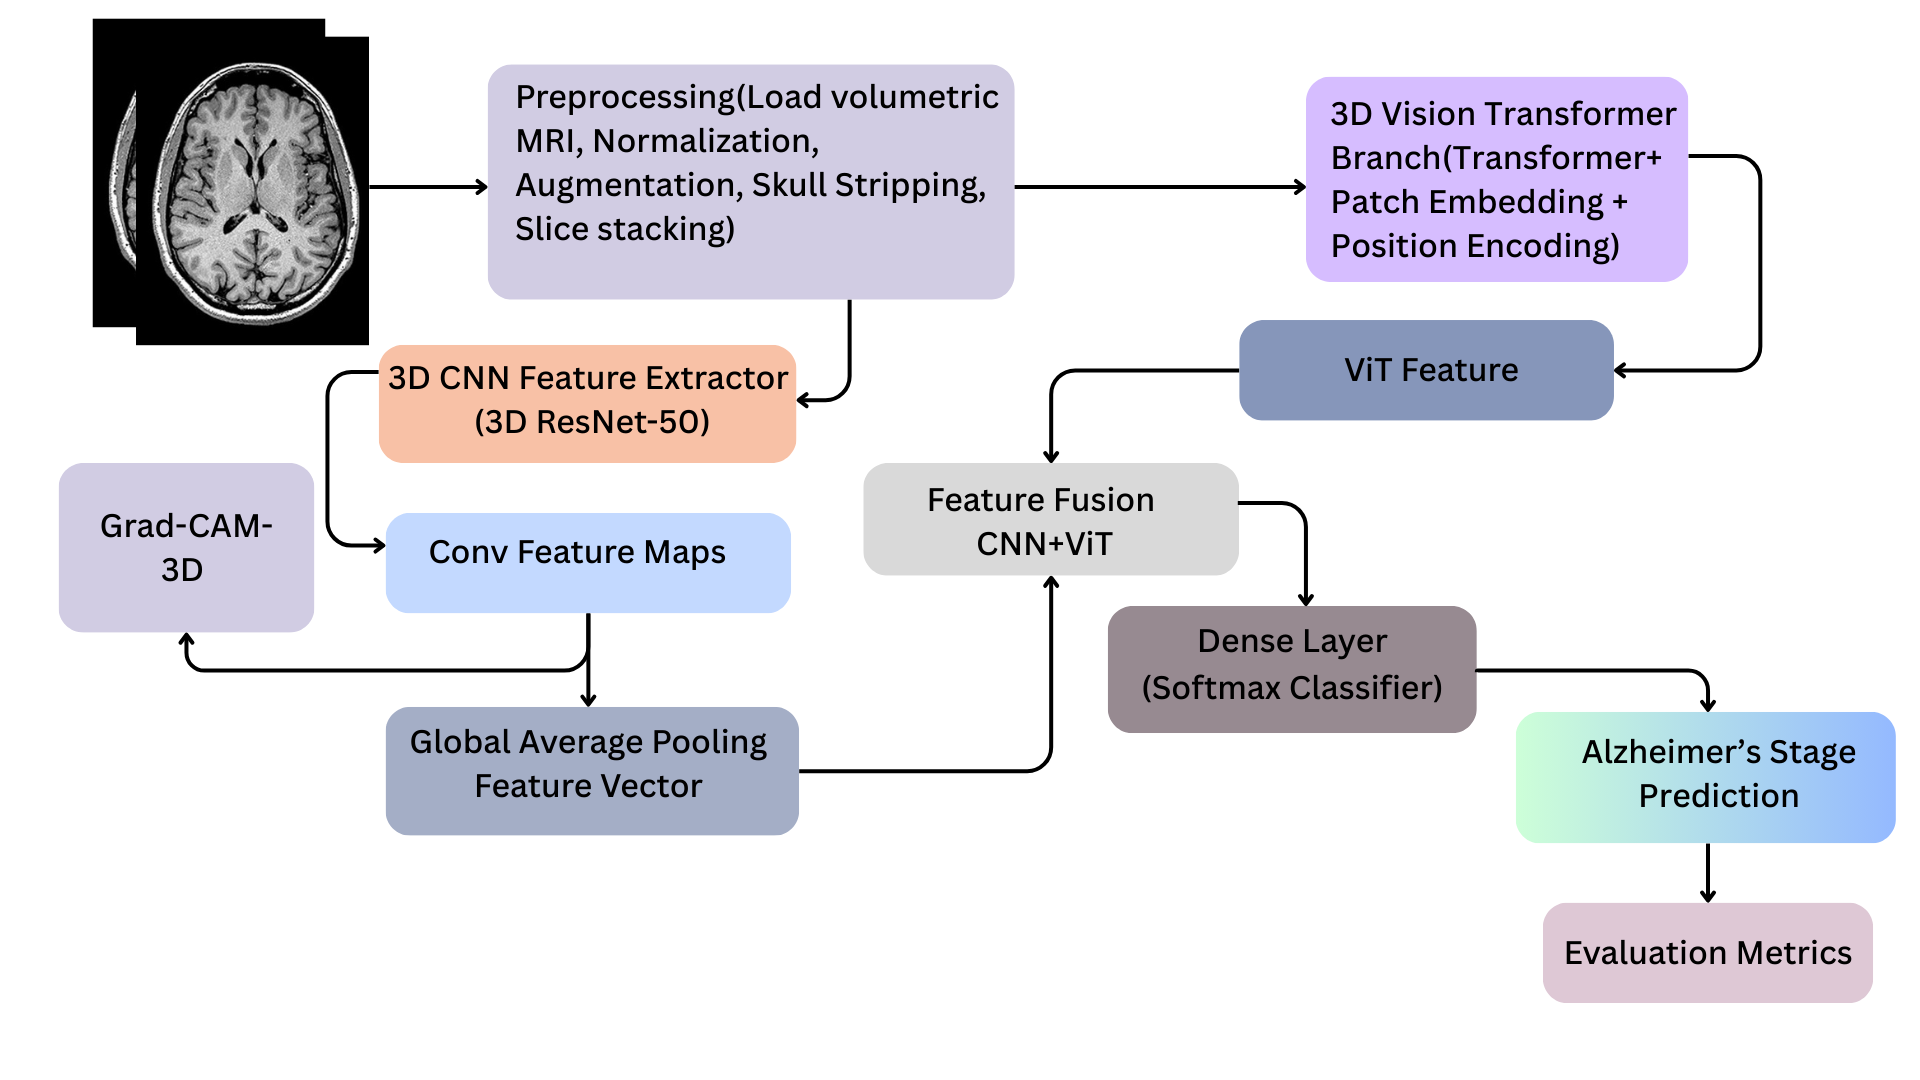
\includegraphics[width=15cm]{Images/Methodology_diagram.png}
    \caption[Methodology overview]{\textbf{Methodology overview.} End-to-end study workflow: problem formulation, single-source ADNI acquisition, deterministic MONAI preprocessing, five 3D architectures sharing a common classifier head, subject-level five-fold training and evaluation reported as mean\,$\pm$\,std, and 3D explainability.}
    \label{fig:methodology}
\end{figure}

\section{Tools, Libraries, and Technologies Used}
The system was implemented entirely in Python using the PyTorch + MONAI stack for 3D medical imaging. The primary tools are:\\
\textbf{Programming Language}: Python 3.10.\\
\textbf{Deep Learning Frameworks}:
\begin{enumerate}
    \item PyTorch 2.11 (CUDA 12.8)~\cite{paszke2019pytorch} --- 3D model implementation, mixed-precision training loops, GPU optimization.
    \item MONAI 1.6~\cite{cardoso2022monai} --- medical-imaging transforms, cached datasets, and the 3D backbone implementations (DenseNet121, ResNet, ViT, SwinUNETR encoder).
\end{enumerate}
\textbf{Supporting Libraries}:\\
NumPy 1.26, SciPy --- numerical operations.\\
NiBabel 5.4 --- reading NIfTI (.nii) MRI volumes.\\
scikit-learn 1.4 --- evaluation metrics (F1, ROC-AUC, confusion matrices) and cross-validation utilities.\\
Matplotlib, Seaborn, scikit-image --- visualization and explainability overlays.\\
TensorBoard --- per-run training curves; results also logged to CSV/JSON.\\
\textbf{Development Environment}: local workstation with VS Code; experiments are fully config-driven (one YAML per run) for reproducibility.\\
\textbf{Hardware}: a single NVIDIA GeForce RTX 5060 Ti (16 GB VRAM), 32 GB system RAM, SSD storage. The 16 GB VRAM budget is the binding constraint that drives several design choices below (input resolution, batch size, gradient accumulation).

\section{Dataset Description}
This study uses the \textbf{ADNI} dataset~\cite{jack2008adni,petersen2010adni} exclusively (ADNI GO/2/3, 3T, 3D T1-weighted MPRAGE, pre-processed N3m NIfTI volumes). Using a single, curated source --- rather than pooling ADNI with slice-based datasets such as MIRIAD or Kaggle --- keeps the labels, modality, and acquisition consistent and makes the subject-level split enforceable.

\subsection{ADNI (Alzheimer's Disease Neuroimaging Initiative)}
ADNI is one of the most widely used and authoritative neuroimaging resources for dementia research, providing T1-weighted 3D MRI collected across multiple sites, scanners, and longitudinal timepoints.\\
Source: ADNI (adni.loni.usc.edu)\\
Scan Type: 3D T1-weighted MPRAGE (GradWarp, N3m corrected)\\
Diagnostic groups used: CN, MCI, AD\\
Field strength: 3T\\
Native resolution: $\sim$256$\times$256$\times$170 voxels ($\sim$1\,mm isotropic)\\
Attributes: subject ID, group, sex, age, acquisition description.

\subsection{Curation and Class Distribution}
The raw export was cleaned to one row per usable scan. \textbf{18 scans (from 9 subjects) were removed}: the \textit{HarP 135} files are hippocampus \emph{segmentations} rather than whole-brain MRI, and the \textit{HHP AC-PC registered} files follow an off-pipeline protocol; those 9 subjects retain their standard N3m scans, so no subject is lost. The curated cohort is summarized in Table~\ref{tab:dataset}.

\begin{table}[H]
\centering
\caption{ADNI cohort after curation (subject-level and scan-level counts).}
\label{tab:dataset}
\begin{tabular}{|l|c|c|c|c|}
\hline
\textbf{Group} & \textbf{Subjects} & \textbf{Scans} & \textbf{Binary task} & \textbf{3-class task} \\
\hline
CN (Cognitively Normal) & 206 & 627 & \checkmark & \checkmark \\
MCI (Mild Cognitive Impairment) & 80 & 182 & --- & \checkmark \\
AD (Alzheimer's Disease) & 109 & 323 & \checkmark & \checkmark \\
\hline
\textbf{Total (3-class)} & \textbf{395} & \textbf{1{,}132} & & \checkmark \\
\textbf{Total (binary, CN+AD)} & \textbf{315} & \textbf{950} & \checkmark & \\
\hline
\end{tabular}
\end{table}

The dataset is \emph{imbalanced} (CN is the majority; MCI is the minority at only 80 subjects), which motivates the use of class-weighted / focal loss and macro-F1 as the primary metric. Several subjects contribute multiple longitudinal scans, which makes the subject-level split (below) essential. Each scan inherits its subject's diagnostic group. \authortodo{confirm whether the group is the baseline (screening) diagnosis or the diagnosis at each visit, and report the follow-up span. If baseline labels are used, a CN or MCI subject who converted at a later visit keeps the old label on later scans, which adds label noise. Also confirm whether the 180 subjects with exactly four scans have four visits, or repeat acquisitions (MPRAGE and MPRAGE-repeat) within fewer sessions.}

\subsection{Exploratory Data Analysis}
Figure~\ref{fig:ds_stats} summarizes the cohort: the class balance (per subject and per scan), the age and sex distributions, and the number of scans per subject. The distributions confirm the expected demographics of an AD cohort (older, with a mild sex skew) and the strong CN/AD-vs-MCI imbalance. AD subjects are on average older than CN subjects (the age densities peak at roughly 76 and 70 years respectively), so age is a potential confounder of atrophy-based classification; this is discussed under Threats to Validity in Chapter~\ref{cha:results}. Figure~\ref{fig:ds_samples} shows representative axial, coronal, and sagittal slices of a CN and an AD subject; the enlarged ventricles and reduced medial-temporal volume in the AD example are visible even to the eye, and are precisely the structural cues the models are expected to learn.

\begin{figure}[H]
    \centering
    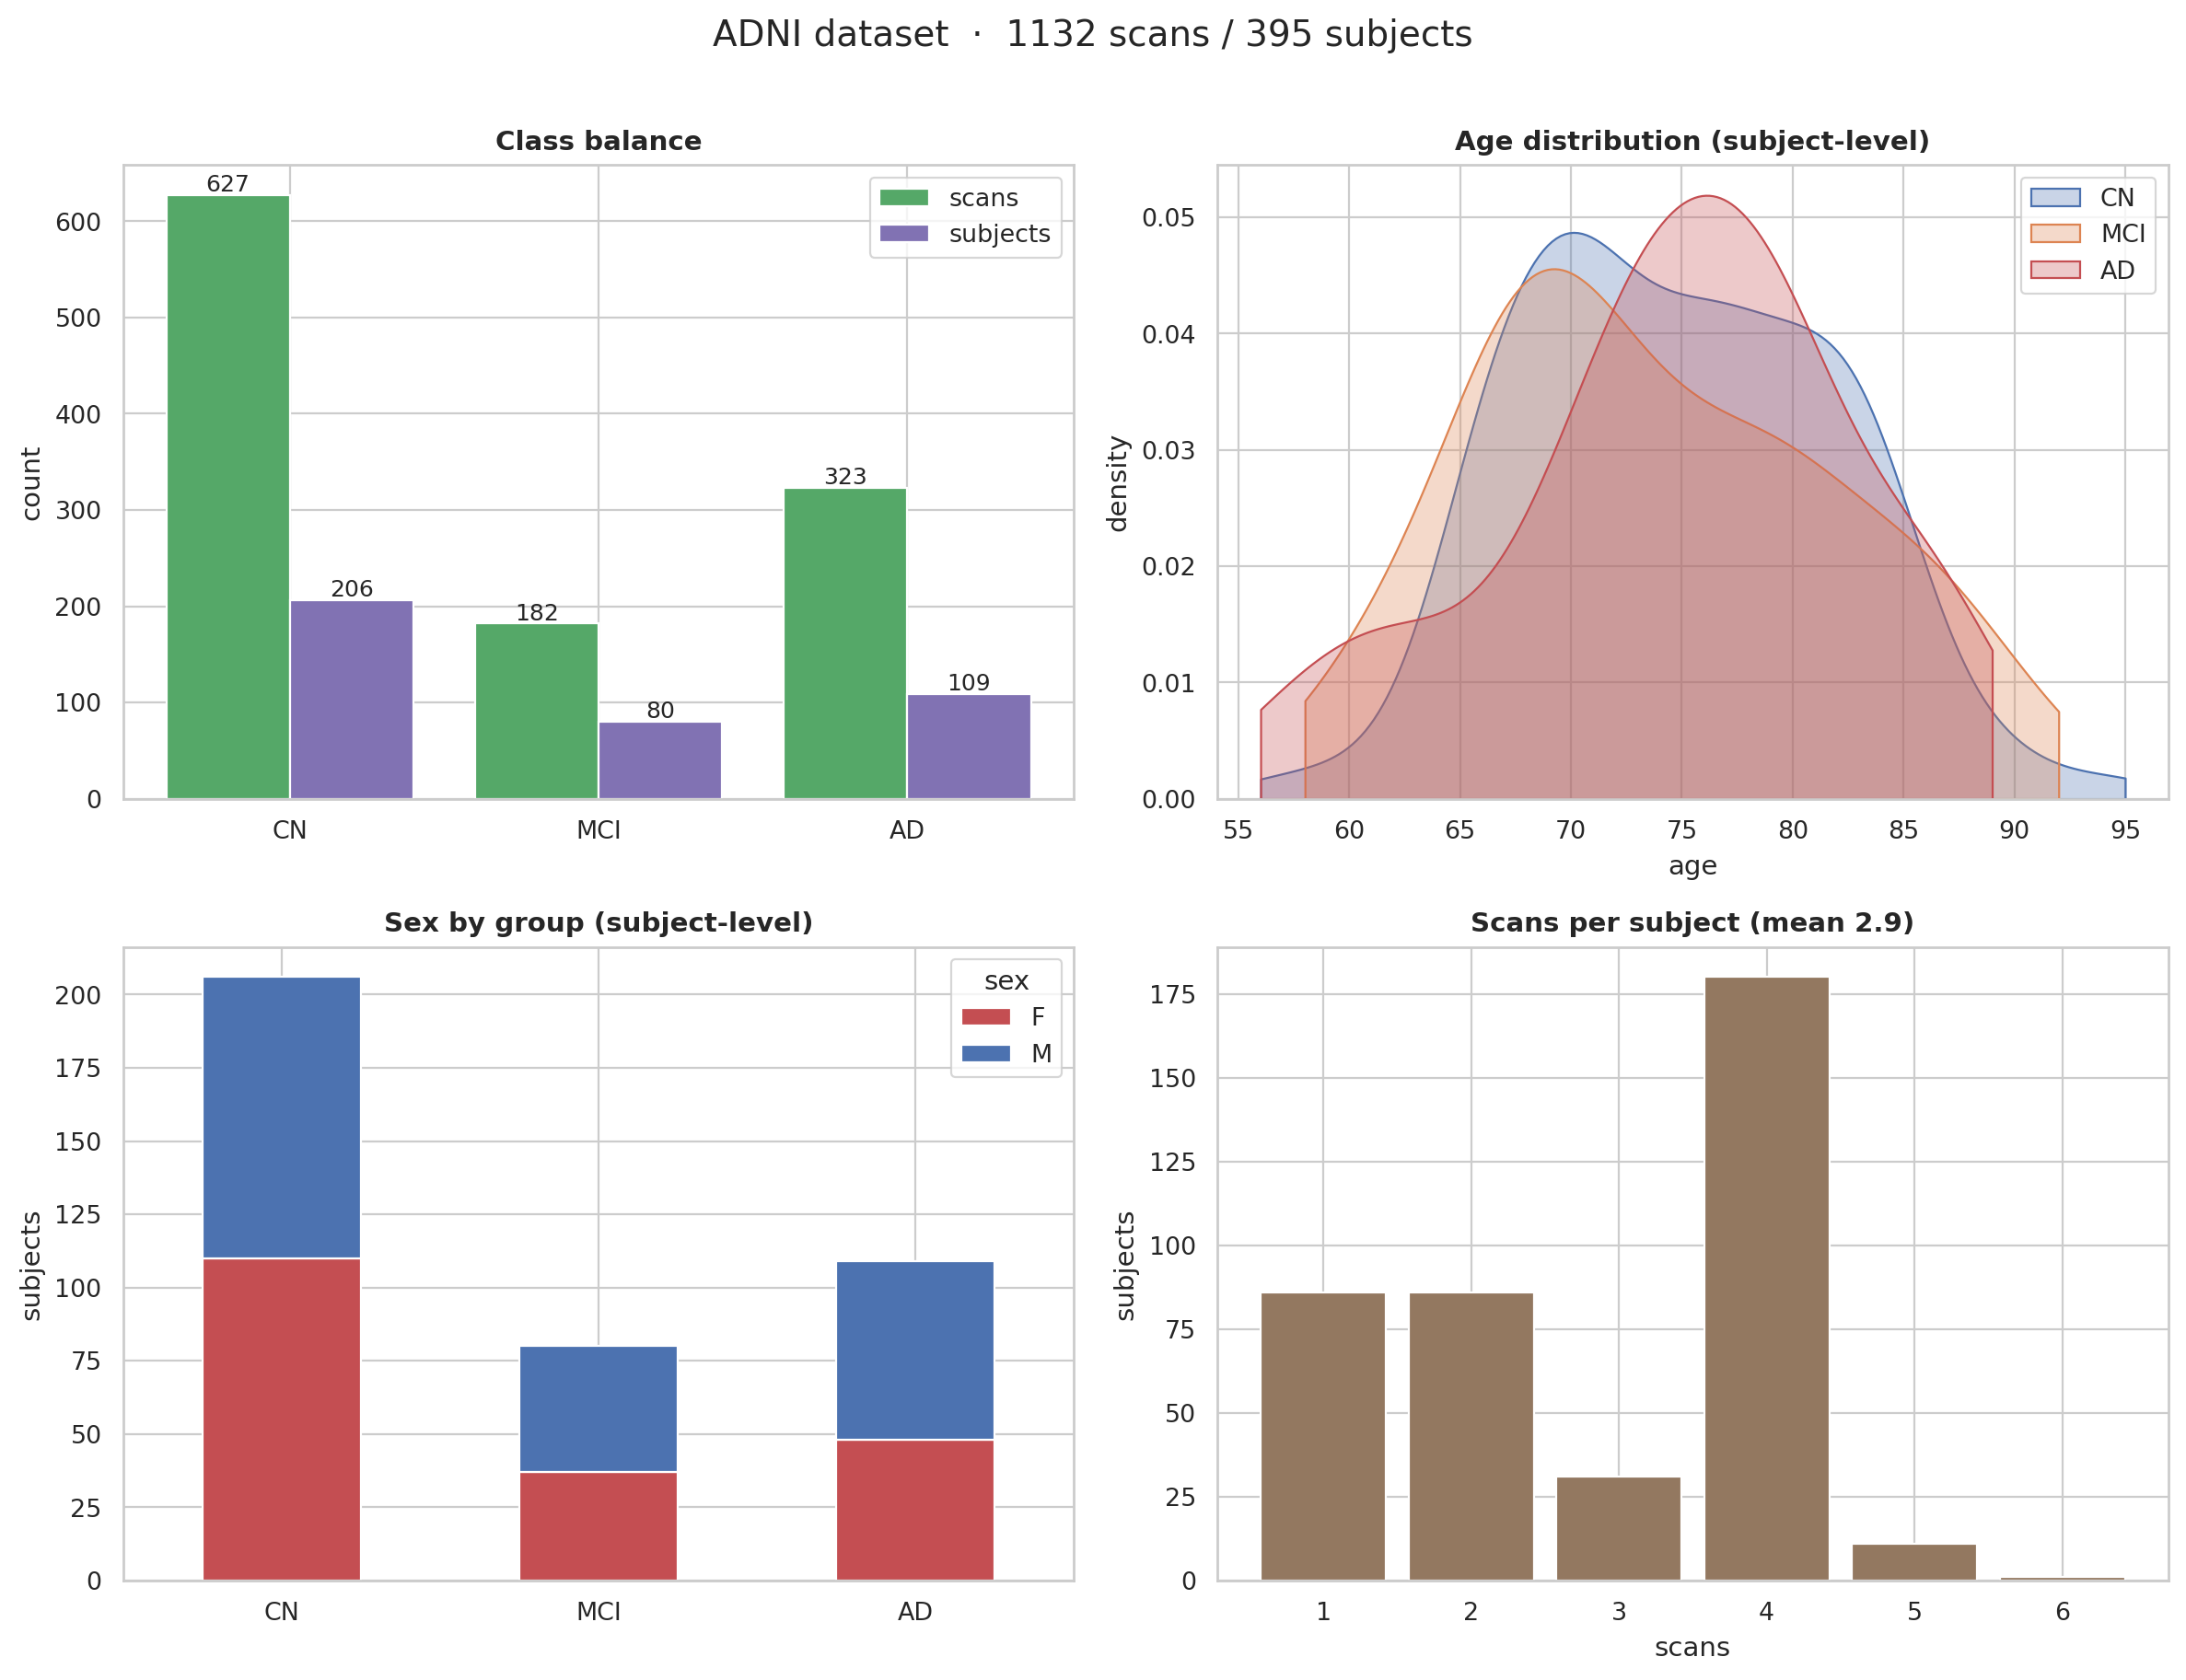
\includegraphics[width=15cm]{Images/ds_stats.png}
    \caption[Cohort statistics]{\textbf{Cohort statistics.} ADNI class balance, age/sex demographics, and scans per subject.}
    \label{fig:ds_stats}
\end{figure}

\begin{figure}[H]
    \centering
    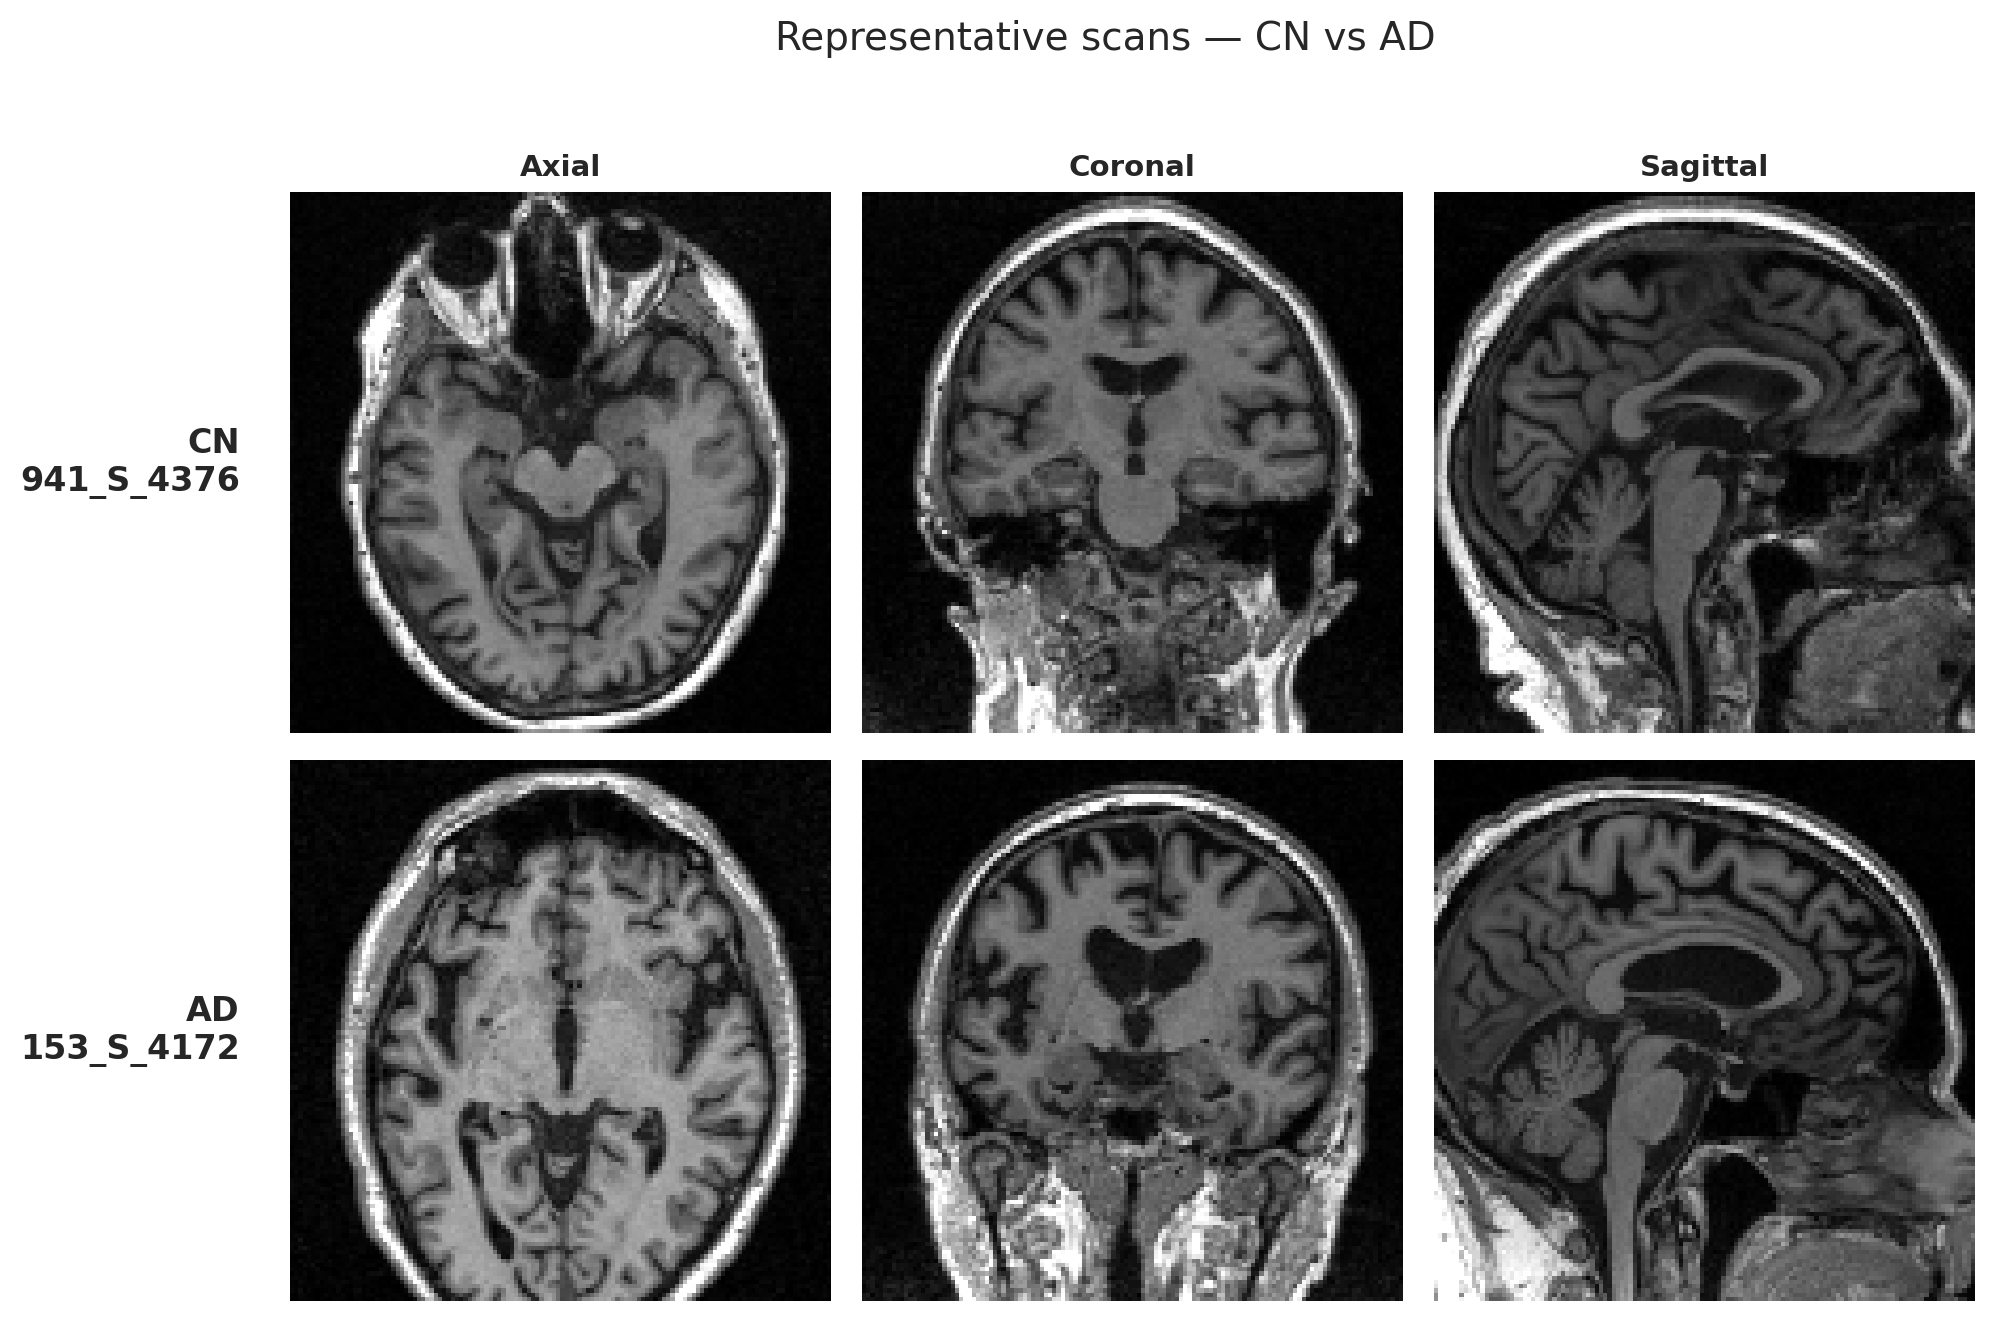
\includegraphics[width=14cm]{Images/ds_samples.png}
    \caption[CN vs.\ AD samples]{\textbf{CN vs.\ AD samples.} Representative preprocessed volumes of a cognitively normal (CN) and an Alzheimer's (AD) subject across the three anatomical planes.}
    \label{fig:ds_samples}
\end{figure}

\subsection{Evaluation Protocol (Subject-Level, Leakage-Free)}
The single most important methodological decision is that \textbf{no subject's scans are ever split across training and testing}. This is enforced and asserted in code (\texttt{build\_dataset.py}). Concretely:
\begin{itemize}
    \item \textbf{Subject-level stratified 5-fold cross-validation} is the primary protocol; a 70/15/15 subject-level hold-out split is also provided. Both use \texttt{seed = 42} and are identical for every model, so comparisons are fair.
    \item \textbf{Two-level metrics.} Each scan is scored (scan-level); in addition, the softmax logits of a subject's multiple scans are averaged into one subject-level prediction --- the clinically meaningful number, and a legitimate, leakage-free boost of a few points.
    \item \textbf{Metrics.} Accuracy, \textbf{macro-F1 (primary, due to imbalance)}, weighted-F1, per-class precision/recall/F1, confusion matrices, and ROC-AUC (one-vs-rest for the three-class task).
    \item \textbf{Model selection / early stopping} is on validation subject-level macro-F1, never on accuracy. \authortodo{state exactly which subjects form the validation set inside each fold. If the held-out test fold itself was used for early stopping, say so here and in the Threats to Validity, because selecting the best epoch on the test fold biases the reported scores upward; the preferred fix is an inner validation split carved from the four training folds.}
    \item \textbf{Reference baseline.} Every table is read against the majority-class baseline --- always predicting CN --- which scores $206/315 = 65.4\%$ accuracy on the binary task and $206/395 = 52.2\%$ on the three-class task. Accuracy is only meaningful in excess of these figures, which is a further reason for using macro-F1.
\end{itemize}
This protocol is deliberately conservative: it produces lower numbers than slice-level splitting, but numbers that would survive scrutiny on unseen patients~\cite{wen2020convolutional,yagis2021effect}.

\section{Preprocessing Steps}
A single deterministic MONAI pipeline is applied identically to train, validation, and test volumes (augmentation is train-only). Steps:\\
\textbf{Load \& channel-first:} read NIfTI, add a channel dimension.\\
\textbf{Orientation:} reorient to canonical RAS axes.\\
\textbf{Resampling:} resample to 1.5\,mm isotropic spacing for a consistent physical scale.\\
\textbf{Foreground crop:} \texttt{CropForeground} removes empty background around the head.\\
\textbf{Intensity normalization:} per-volume z-score normalization over non-zero voxels.\\
\textbf{Resize / pad:} to a fixed cubic tensor --- $96^3$ for every binary run and for the three-class ViT, and $128^3$ for the three-class CNN and Swin (Appendix~\ref{app:repro}); the transformer patch-embedding and the 16\,GB VRAM budget make $96^3$ the practical size for the hybrids.\\
\textbf{Caching:} a MONAI \texttt{CacheDataset} computes this deterministic pipeline once and reuses it, giving a large speed-up on the small cohort.\\[4pt]
\textbf{Note on skull-stripping.} The ADNI N3m volumes are \emph{not} skull-stripped, and this pipeline does not strip them by default; brain extraction and MNI registration are treated as optional ablations rather than a fixed step. This is stated explicitly because it affects how the explainability maps in Chapter~\ref{cha:results} are interpreted (importance is reported over coarse spatial regions of the head volume, not atlas ROIs).\\[4pt]
\textbf{Data Augmentation (train only):} random flips, random affine ($\pm10^{\circ}$ rotation, mild scaling/translation), Gaussian noise and smoothing, random bias field, gamma/contrast adjustment, and intensity scale/shift. These act as strong regularizers on a small dataset.

Figure~\ref{fig:preproc} illustrates the deterministic preprocessing pipeline applied to every volume, and Figure~\ref{fig:augment} shows examples of the stochastic training-time augmentations.

\begin{figure}[H]
    \centering
    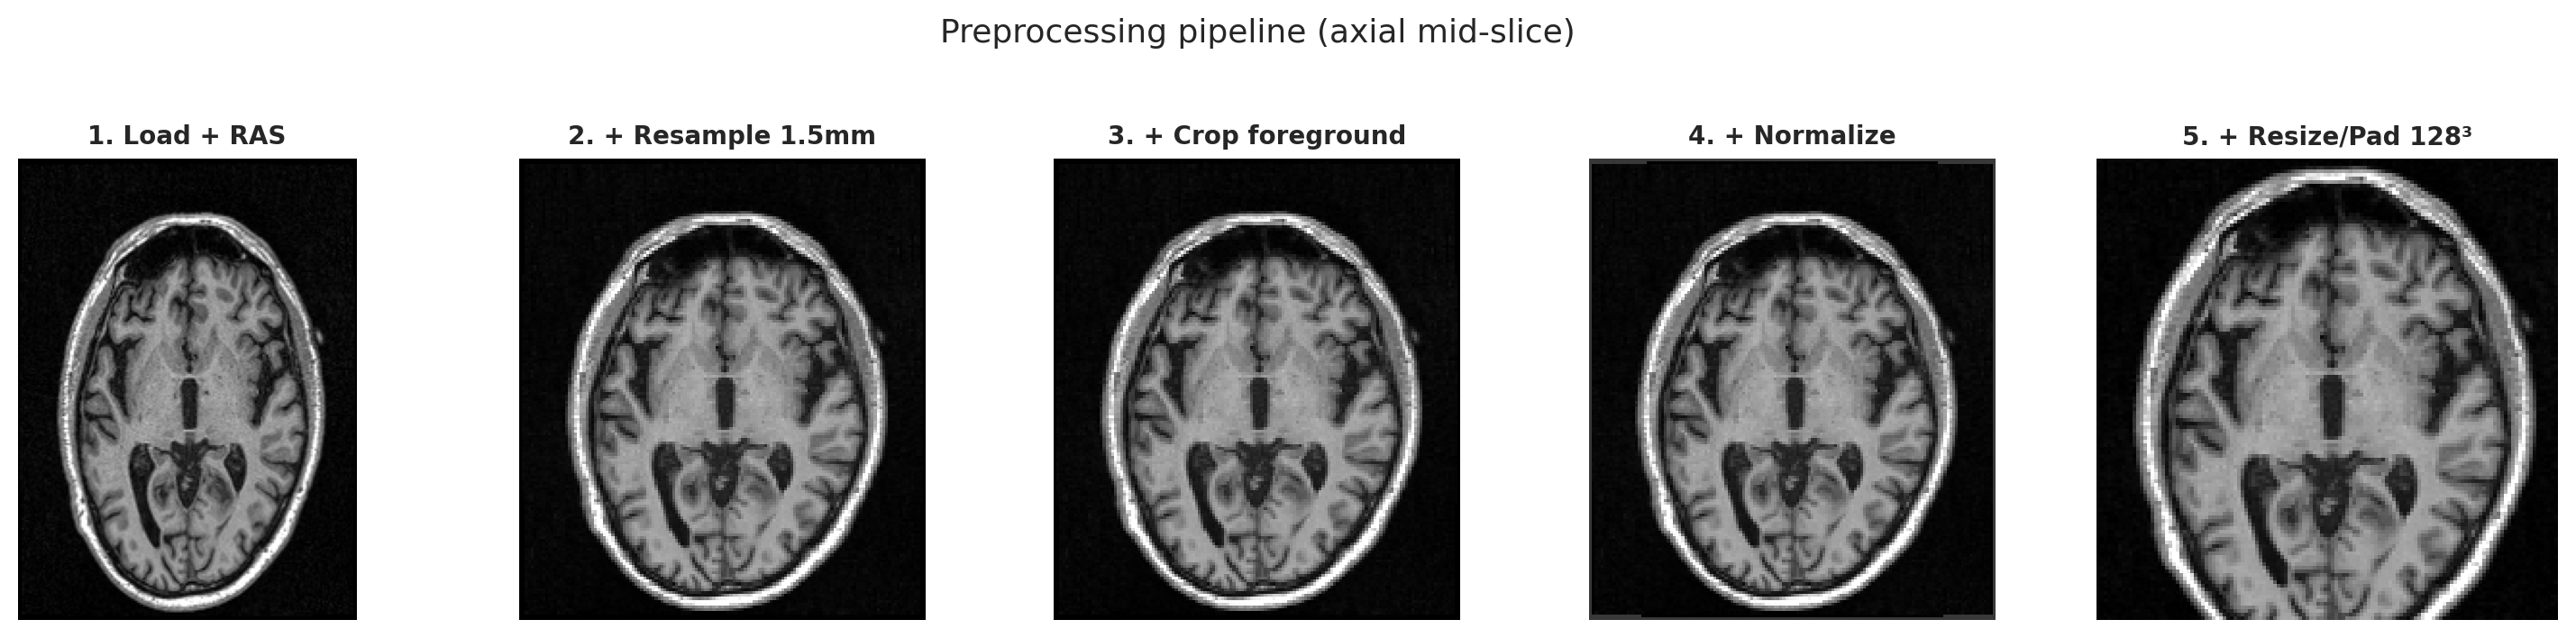
\includegraphics[width=15cm]{Images/ds_preprocessing.png}
    \caption[Preprocessing pipeline]{\textbf{Preprocessing pipeline.} Deterministic steps applied to every volume: reorientation, resampling, foreground crop, z-score normalization, and resizing.}
    \label{fig:preproc}
\end{figure}

\begin{figure}[H]
    \centering
    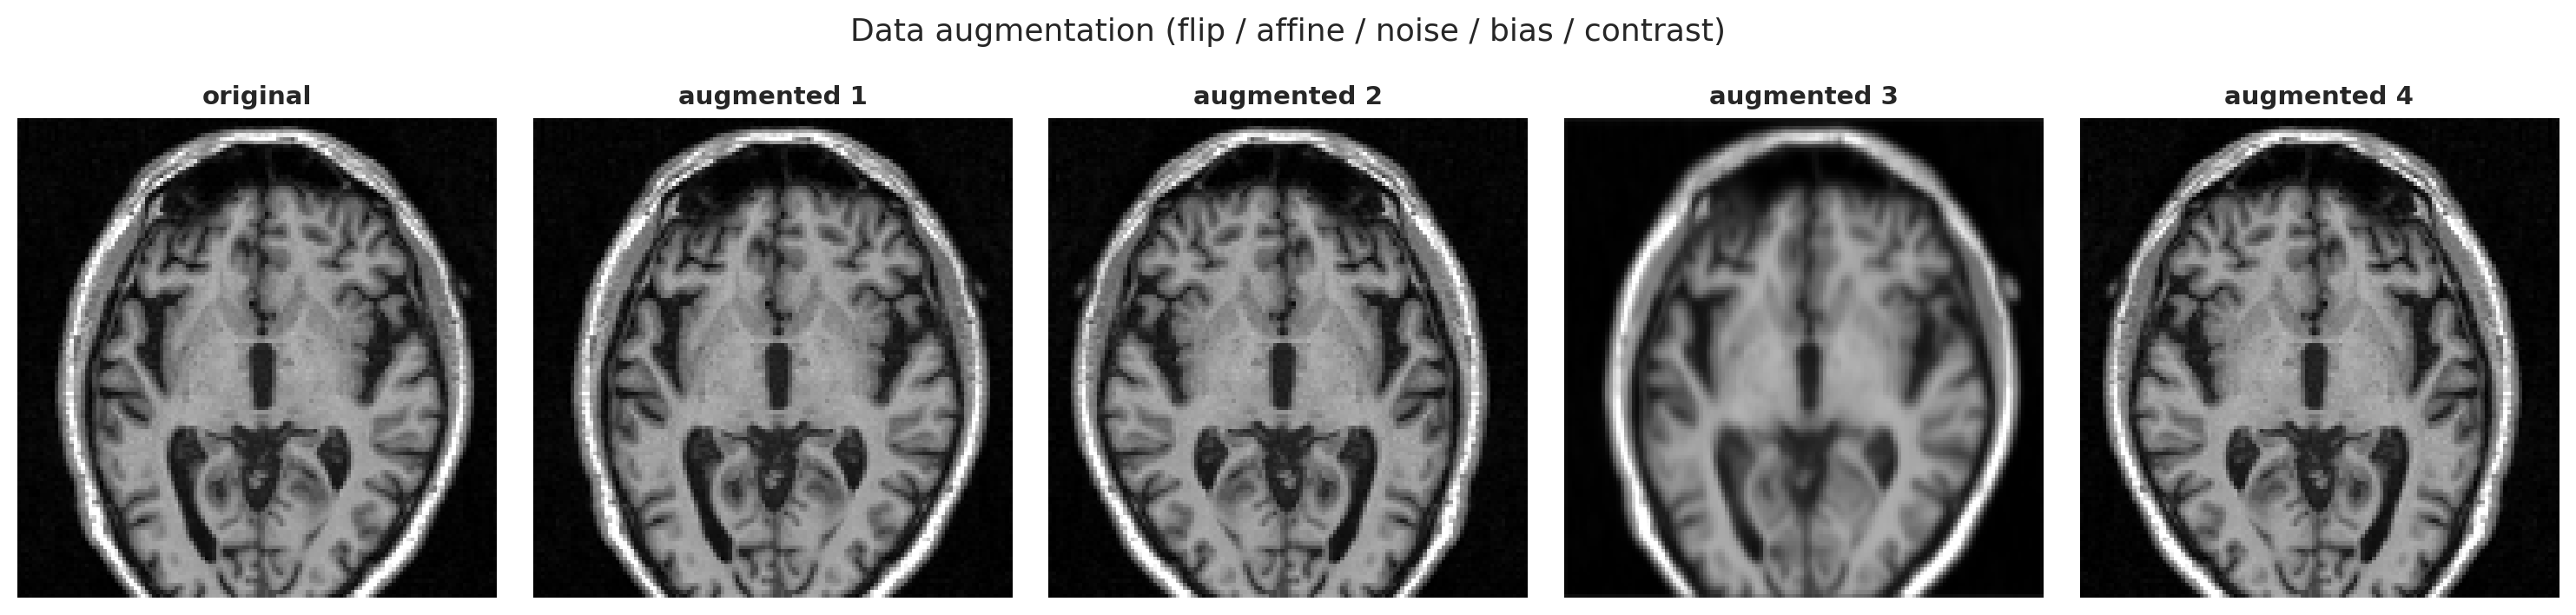
\includegraphics[width=14cm]{Images/ds_augmentation.png}
    \caption[Training augmentations]{\textbf{Training augmentations.} Examples of the training-only 3D augmentations (flips, affine, noise, intensity perturbations).}
    \label{fig:augment}
\end{figure}

\section{Model Development / Algorithm Design}
Five 3D backbones (and two hybrid combinations of them) are implemented behind a \emph{common interface}: every backbone exposes \texttt{forward\_features(x)} returning a $(B, \text{feat\_dim})$ vector, and a shared dropout + linear classifier head maps it to the class logits. Because the head and the training recipe are identical, the single-vs-hybrid comparison is genuinely apples-to-apples.

\subsection{Standalone Backbones}
\textbf{(1) 3D CNN --- DenseNet-121}~\cite{huang2017densely} (MONAI, trained from scratch). Densely connected 3D convolutions extract hierarchical local features (cortical thinning, ventricular enlargement, hippocampal atrophy); global-average pooling yields a 1024-D feature vector. This is the primary CNN baseline.\\
\textbf{(2) 3D ResNet --- MedicalNet pretrained.} A 3D ResNet~\cite{he2016deep} initialized with Tencent MedicalNet weights~\cite{chen2019med3d} (pretrained on 23 medical datasets) to test whether medical transfer learning helps on this cohort. It produces a 512-D feature vector.\\
\textbf{(3) 3D Vision Transformer (ViT)}~\cite{dosovitskiy2021image}. A compact ViT (hidden size 384, 6 layers, 6 heads, $16^3$ patch embedding on a $96^3$ input), trained from scratch, with token-average pooling. It tests how a pure global-attention model behaves on a small 3D dataset.\\
\textbf{(4) Swin Transformer}~\cite{liu2021swin,hatamizadeh2021swinunetr}. The hierarchical SwinUNETR-style encoder (shifted-window attention, embedding dim 48, four stages), with global-average pooling of the deepest stage. It is a strong, data-efficient transformer option for 3D medical imaging.

\subsection{Hybrid 3D CNN--ViT (Proposed)}
The proposed model runs two backbones in parallel on the same volume and fuses their features:
\begin{itemize}
    \item the \textbf{3D CNN branch} contributes local, texture-level anatomical detail;
    \item the \textbf{3D ViT branch} contributes global, long-range structural context.
\end{itemize}
Two fusion strategies are supported: \textbf{late concatenation} (the two feature vectors are concatenated and passed to the head) and \textbf{cross-attention} (the CNN feature attends to the transformer feature via a multi-head attention block). The fused representation goes through the shared dropout + linear head and a softmax. This design directly operationalizes the research question of whether combining local and global 3D features beats either alone. Algorithm~\ref{alg:hybrid} sketches the forward pass. Only late-concatenation fusion was trained and evaluated in this thesis; cross-attention is implemented but left to future work.

As a control for the role of the CNN branch, a second hybrid, \textbf{Swin--ViT}, fuses the Swin encoder (in place of DenseNet) with the same ViT branch by late concatenation. It contains no convolutional branch, so comparing it with CNN--ViT indicates how much of the hybrid's signal comes from the CNN. Because it differs from CNN--ViT in its first branch rather than in the fusion mechanism, it is a comparison of \emph{branch choice}, not of fusion strategy.

\begin{algorithm}[H]
\caption{Hybrid 3D CNN--ViT classification (late-concat fusion)}
\label{alg:hybrid}
\begin{algorithmic}[1]
\Require Preprocessed MRI volume $V \in \mathbb{R}^{1\times96\times96\times96}$
\Ensure Class prediction $\hat{y}$ and 3D importance map $H$
\State $f_{\text{cnn}} \gets \textsc{DenseNet3D.forwardFeatures}(V)$ \Comment{local features, 1024-D}
\State $f_{\text{vit}} \gets \textsc{ViT3D.forwardFeatures}(V)$ \Comment{global features, 384-D}
\State $z \gets \textsc{Concat}(f_{\text{cnn}}, f_{\text{vit}})$
\State $\text{logits} \gets \textsc{Linear}(\textsc{Dropout}(z))$
\State $\hat{y} \gets \textsc{Softmax}(\text{logits})$
\State $H \gets \textsc{GradCAM3D}(f_{\text{cnn}})$ \Comment{explainability overlay}
\State \Return $\hat{y}, H$
\end{algorithmic}
\end{algorithm}

\section{Training Recipe}
Within each task, all models share one recipe so that differences reflect the architecture, not the tuning (the binary and three-class recipes differ in loss, epochs, warmup, patience, and weight decay; the exact values per run are listed in Appendix~\ref{app:repro}):
\begin{itemize}
    \item \textbf{Optimizer:} AdamW~\cite{loshchilov2019decoupled}, learning rate $1\times10^{-4}$, weight decay $0.01$--$0.03$.
    \item \textbf{Schedule:} cosine decay~\cite{loshchilov2017sgdr} with linear warmup (5--8 epochs), up to 80--100 epochs.
    \item \textbf{Loss:} focal loss~\cite{lin2017focal} ($\gamma=2$) for the three-class task (to handle the MCI minority); class-weighted cross-entropy with label smoothing~\cite{muller2019does} $0.1$ for the binary task. Class weights / weighted sampling address imbalance. \authortodo{state exactly which imbalance corrections were active in each run --- class-weighted loss, weighted sampler, focal loss, or a combination. Stacking several corrections can over-correct towards the minority classes, which is relevant to the three-class ViT result in Chapter~\ref{cha:results}.}
    \item \textbf{Memory:} automatic mixed precision (AMP) + gradient accumulation (batch size 2, accumulation 4 $\rightarrow$ effective batch 8) + gradient clipping at 1.0, to fit 3D volumes in 16\,GB.
    \item \textbf{Regularization:} dropout (0.2), weight decay, heavy 3D augmentation, and early stopping on validation subject-level macro-F1 (patience 15--18).
    \item \textbf{Reproducibility:} every run seeds all RNGs, logs library versions, and saves its exact YAML config, the split file, per-fold metrics, and checkpoints.
\end{itemize}

\section{System Implementation / Modules Description}
The system is modular. The \textbf{Data module} indexes ADNI volumes by image-ID, builds subject-level loaders and the weighted sampler, and applies the MONAI transforms. The \textbf{Model module} contains the five backbones, the shared classifier head, and the hybrid fusion blocks behind the common \texttt{build\_model(cfg)} factory. The \textbf{Training module} runs AMP training, tracks validation subject-level macro-F1, early-stops, and checkpoints. The \textbf{Evaluation module} computes scan- and subject-level metrics, confusion matrices, and ROC curves, and aggregates folds into mean $\pm$ std summaries. The \textbf{Explainability module} generates Grad-CAM/Grad-CAM++/Integrated-Gradients/attention-rollout overlays for a chosen model and subject.

\section{Hardware and Software Requirements}
\textbf{Hardware.} Training was performed on a single NVIDIA RTX 5060 Ti (16\,GB), 32\,GB RAM. The 16\,GB budget dictates $96^3$--$128^3$ inputs, batch size 2 with gradient accumulation, and AMP. Inference (including explainability) runs comfortably on the same GPU.\\
\textbf{Software.} Python 3.10, PyTorch 2.11 (CUDA 12.8), MONAI 1.6, NiBabel 5.4, scikit-learn 1.4, NumPy 1.26, under Windows with an NVIDIA CUDA 12.x driver. All frameworks are open-source.

\section{Summary}
This chapter described the complete, reproducible methodology: a curated single-cohort (multi-site) ADNI dataset (1{,}132 scans / 395 subjects) evaluated under a strict subject-level five-fold protocol; a deterministic MONAI preprocessing pipeline; five 3D architectures sharing one interface, head, and training recipe; and a hybrid 3D CNN--ViT as the proposed model. The design prioritizes a fair, leakage-free comparison over headline accuracy, setting up the experimental results reported in Chapter~\ref{cha:results}.
